\documentclass{standalone}
\usepackage{tikz}
\usepackage{ctex,siunitx}
\setCJKmainfont{Noto Serif CJK SC}
\usepackage{tkz-euclide}
\usepackage{amsmath}
\usetikzlibrary{patterns, calc}
\usetikzlibrary {decorations.pathmorphing, decorations.pathreplacing, decorations.shapes,}
\begin{document}
\small
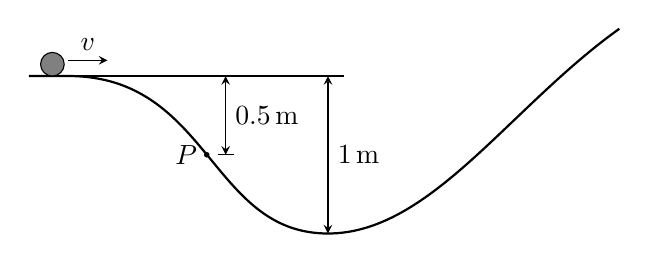
\begin{tikzpicture}[>=stealth,scale=1]
  \draw[thick](-0.5,2)--(0,2)..controls(1.8,2)and(1.8,0)..(3.3,0)..controls(4.6,0)and(5.6,1.6)..(7,2.6);
  \draw [->] (0,2.2)--++(0.5,0)node[midway,above]{$v$};
  \draw [fill=gray](-0.2,2.15) circle (.15);
  \draw [thin](0.1,2)--(3.5,2);
  \draw [thin](1.9,1)--(2.1,1);
  \draw [thin,<->](3.3,0)--(3.3,2)node[midway,right]{\qty{1}{m}};
  \draw [thin,<->](2.0,1)--(2.0,2)node[midway,right]{\qty{0.5}{m}};
  \fill (1.76,1) circle(1pt)node[left]{$P$};
\end{tikzpicture}
\end{document}